\documentclass[11pt,a4paper]{article}
\usepackage[margin=25mm,headheight=15pt]{geometry}
\usepackage{amsmath,amssymb,booktabs,tabularx,array}
\usepackage{xcolor,tikz,fancyhdr,enumitem}
\usetikzlibrary{arrows.meta,positioning}
\definecolor{ink}{HTML}{153A50}
\definecolor{accent}{HTML}{087F8C}
\usepackage[unicode,colorlinks=true,linkcolor=accent!75!black,urlcolor=accent!75!black,citecolor=accent!75!black]{hyperref}
\hypersetup{pdftitle={On-Policy Self-Distillation with Privileged Information for Mathematical Reasoning in Language Models under 30B Parameters},pdfauthor={Kai Zhu},pdfsubject={Research Report 1}}
\newcommand{\studentid}{26723810}
\newcommand{\studentname}{Kai Zhu}
\newcommand{\reportdate}{November 27, 2026}
\newcolumntype{Y}{>{\raggedright\arraybackslash}X}
\setlength{\parskip}{0.3em}
\setlength{\emergencystretch}{2em}
\setlist{nosep,leftmargin=2em}
\renewcommand{\arraystretch}{1.22}
\setcounter{tocdepth}{2}
\pagestyle{fancy}
\fancyhf{}
\fancyhead[L]{\small\color{ink}Research Report 1 \enspace|\enspace On-Policy Self-Distillation}
\fancyhead[R]{\small\studentname\enspace\studentid}
\fancyfoot[C]{\small\thepage}
\begin{document}
\hypersetup{pageanchor=false}
\begin{titlepage}
\setlength{\parindent}{0pt}
\vspace*{17mm}
{\large\sffamily\color{accent}FIRST RESEARCH REPORT\par}
\vspace{10mm}
{\Huge\bfseries\color{ink}On-Policy Self-Distillation\\[0.15em]
with Privileged Information\par}
\vspace{5mm}
{\LARGE\color{ink}Mathematical Reasoning in Language Models\\
under 30B Parameters\par}
\vspace{5mm}
{\large Effectiveness, Behavioral Drift, and Reward Calibration\par}
\vspace{15mm}
\begin{tabular}{@{}ll}
Author & \studentname\\
Student ID & \studentid\\
Date & \reportdate\\
Core literature & 10 papers first made public from April to November 2026\\
Model scope & Primarily student models with 0.6B to 14B parameters\\
Report type & Critical literature survey\\
\end{tabular}
\vfill
\noindent\colorbox{ink!6}{\parbox{\dimexpr\linewidth-2\fboxsep\relax}{\small
\textbf{Research question.} When a teacher sees a correct solution during training, does its token-level supervision transfer generalizable reasoning skills, or does it change how the student uses and expresses skills it already has?
\par\medskip
\textbf{Evidence.} The ten core papers are cited as arXiv preprints. The survey draws on their reported experiments. The proposed follow-up experiments have yet to be run.}}
\end{titlepage}
\pagenumbering{roman}
\hypersetup{pageanchor=true}
\section*{Abstract}
On-policy self-distillation with privileged information uses one language model as both teacher and student. During training, the teacher receives additional context such as a reference solution, error feedback, or a revised attempt. The student receives only the original problem, generates its own response, and learns from the teacher's next-token distributions along that response. This approach supplements sparse outcome rewards with dense supervision without requiring a separate large teacher. This survey examines ten studies first made public after January 2026. It focuses on mathematical reasoning in student models below 30 billion parameters and compares revision-based approaches, diagnostics of self-distillation, contrastive supervision, and reward calibration.

The survey distinguishes three questions: whether task performance improves, whether privileged information causes the gain, and whether that gain transfers to new reasoning problems. Each requires different evidence. Reducing the discrepancy between student and teacher distributions alone does not guarantee higher task reward. Access to a solution can also change the teacher's response length, confidence, and reasoning mode. Contrasting correct and incorrect contexts and retaining a reward objective are two approaches that warrant further testing. The survey proposes an experiment with reference ablations, matched reasoning modes and budgets, and independent tests. It also discusses memory and compute costs in small-model implementations.

\noindent\textbf{Keywords:} on-policy self-distillation, privileged information, mathematical reasoning, verifiable rewards, credit assignment, behavioral drift

\medskip
\noindent\textbf{Scope.} The date requirement is interpreted conservatively. All core papers first appeared after January 31, 2026. Papers first released in January are cited as background, including those revised later. The parameter limit applies to the student experiments analyzed here. Individual papers may use larger models for auxiliary tasks, data generation, or additional baselines.

\clearpage
\tableofcontents
\clearpage
\pagenumbering{arabic}

\section{Research Questions and Study Selection}
\subsection{Why Focus on Mathematical Reasoning?}
Mathematics is a useful setting for studying self-distillation because final answers are often easy to verify automatically, while reliable labels for intermediate reasoning steps are difficult and costly to obtain. An outcome reward indicates whether an entire response succeeded, but it gives little guidance about individual tokens in a long derivation. Self-distillation supplies token-level guidance based on differences in teacher and student probabilities. The central technical question is how well those differences track correctness.

The scope is the intersection of autoregressive language models, token-level supervision on student-generated trajectories, and performance and attribution in mathematical reasoning. Findings from coding, logic puzzles, and tool use are discussed where they clarify a mechanism or its generality. The survey excludes diffusion-model acceleration, visual representation self-distillation, and self-reflection implemented solely through prompting.

\textbf{RQ1.} How is privileged information converted into a parameter update?
\textbf{RQ2.} Which controls distinguish transfer of reasoning skills from transfer of behavior?
\textbf{RQ3.} What problems do contrastive supervision and reward calibration address?
\textbf{RQ4.} How can we compare these methods fairly and feasibly on models below 30B parameters?

\subsection{Search and Inclusion Criteria}
The search ended on \reportdate. Web searches identified original arXiv records. Abstracts, version histories, experimental setups, tables, and relevant analyses were then checked against the papers. Search terms included \texttt{on-policy self-distillation}, \texttt{privileged information}, \texttt{reasoning}, \texttt{contrastive}, and \texttt{2026}. References in the papers led to additional studies. This is a targeted review with stated selection criteria. A complete list of database hits and exclusions was not recorded.

To be included, a study had to meet the date criterion, directly address the research question, offer analyzable student experiments below 30B parameters, describe a method or controlled diagnostic, and provide an accessible original record and experimental account. Study quality was assessed through controls, ablations, evidence across model families, and reporting clarity. The recent preprints have had limited time to accumulate independent replications and citations.

\begin{table}[htbp]
\centering\small
\caption{The ten core studies. P identifiers are used throughout the report. Dates indicate first public release in 2026, and versions identify the manuscripts reviewed. All entries are cited as preprints.}
\label{tab:corpus}
\begin{tabularx}{\linewidth}{@{}lYll@{}}
\toprule
ID & Study and principal models examined & First release & Version\\
\midrule
P1 & SD-Zero. Qwen3-4B and OLMo-3-7B & Apr 13 & v2\\
P2 & RLCSD. Qwen3-1.7/4/8B and OLMo-3-7B & Jun 10 & v2\\
P3 & Privileged, but Biased. Qwen3-8B subset & Aug 5 & v1\\
P4 & What Does PI Add? Qwen3-1.7B and SmolLM3-3B & Sep 17 & v2\\
P5 & Repulsive and Attractive Teachers. Qwen3-4B & Sep 18 & v1\\
P6 & SIPO. Qwen3-8B and OLMo3-7B & Sep 29 & v1\\
P7 & Diagnosing OPSD. Several models from 0.6B to 8B & Sep 30 & v2\\
P8 & Does SD Improve Reasoning? Qwen3-1.7B to 14B and others & Oct 13 & v1\\
P9 & VASPO. Qwen3-4B and OLMo3-7B & Oct 14 & v1\\
P10 & Auditing OPSD. Qwen3-1.7/4/8B & Nov 11 & v1\\
\bottomrule
\end{tabularx}
\end{table}

P3 also reports a 32B question-answering experiment, which is excluded from the small-model evidence. Some P1 baselines use demonstrations generated by external models, so the student parameter count alone cannot establish that their data generation meets the same constraint. The original OPSD and SDPO papers first appeared in January and are cited as background outside the ten-paper corpus \cite{opsd,sdpo}. The references give full titles, version numbers, and links.

\section{Technical Framework}
\subsection{Student Trajectories and the Privileged Teacher}
Let \(x\) be a problem and \(z\) be privileged information available during training. The student samples a response \(y\sim\pi_\theta(\cdot\mid x)\). At each prefix \(y_{<t}\) visited by the student, the next-token distributions are
\begin{equation}
p_t(v)=\pi_\theta(v\mid x,y_{<t}),\qquad
q_t(v)=\pi_{\bar\theta}(v\mid x,z,y_{<t}).
\end{equation}
The teacher parameters \(\bar\theta\) may be frozen, periodically synchronized, or updated using an exponential moving average. The teacher and student can start with the same architecture and tokenizer while receiving different contexts. Depending on the implementation, training may still require separate weight copies, and the two conditional distributions can exhibit different capabilities.

A schematic objective using reverse KL divergence is
\begin{equation}
\mathcal L_{\rm SD}=\mathbb E_{x,y\sim\pi_\theta}
\left[\frac{1}{|y|}\sum_t
D_{\rm KL}\bigl(p_t\|\operatorname{sg}(q_t)\bigr)\right],
\label{eq:sd}
\end{equation}
where \(\operatorname{sg}\) stops gradients through the teacher target. Equation~\eqref{eq:sd} illustrates the conditional distributions and the source of trajectories. Implementations also use Jensen--Shannon divergence (JSD), token selection, clipping, or different normalizations. A local divergence loss on sampled student prefixes and an objective differentiated through the trajectory sampling distribution can yield different updates.

Reinforcement learning with verifiable rewards instead optimizes expected task outcomes:
\begin{equation}
J_R(\theta)=\mathbb E_{y\sim\pi_\theta(\cdot\mid x)}R(x,y),\qquad
R(x,y)\in\{0,1\}.
\end{equation}
An outcome-based method often assigns the same response-level advantage to many tokens. That advantage provides a direction for the whole response, with limited information about which step helped. Self-distillation supplies local preferences, which need not track the chance that the student's continuation produces a correct answer.

\begin{figure}[htbp]
\centering
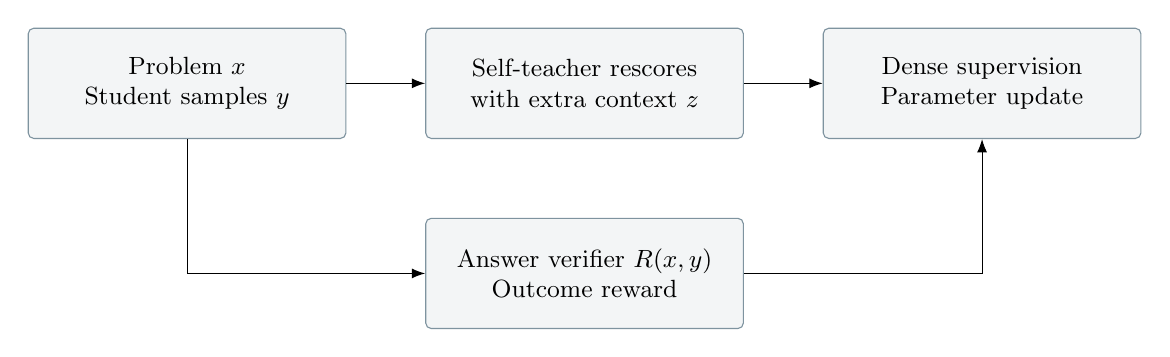
\begin{tikzpicture}[>=Latex,node distance=10mm,
box/.style={draw=ink!55,rounded corners=2pt,fill=ink!5,align=center,text width=38mm,minimum height=14mm,font=\small}]
\node[box] (x) {Problem \(x\)\\Student samples \(y\)};
\node[box,right=of x] (q) {Self-teacher rescores\\with extra context \(z\)};
\node[box,right=of q] (loss) {Dense supervision\\Parameter update};
\node[box,below=of q] (r) {Answer verifier \(R(x,y)\)\\Outcome reward};
\draw[->] (x)--(q);
\draw[->] (q)--(loss);
\draw[->] (x.south)|-(r.west);
\draw[->] (r.east)-|(loss.south);
\end{tikzpicture}
\caption{Common training flow. The reward branch participates in the update for methods that use it. Independent student testing uses the original problem alone.}
\end{figure}

\subsection{Three Criteria for Success}
\textbf{Performance.} The trained student outscores the initial model on a test set.
\textbf{Attribution.} A teacher with privileged information outperforms a matched teacher without it, with reasoning mode, trajectories, budgets, and prompt templates controlled.
\textbf{Transfer.} The gain persists on unseen problems at matched reasoning modes and token budgets. Each successive criterion requires additional evidence.

Consider a base model that scores 20\% in short-answer mode and 50\% in extended reasoning mode. If training raises its short-answer score to 40\%, it improves that deployment setting. The experiment leaves open whether the model acquired a capability beyond what its original extended reasoning mode could already deliver. These figures are illustrative.

\section{Contributions and Limits of the Ten Core Studies}
The studies below are grouped by the question they help answer. Each discussion describes a reported finding and evaluates what the experiment supports.

\subsection{Constructing Privileged Information from Rewards}
\textbf{P1. SD-Zero \cite{p1}.} This method first trains a model to revise its initial answers using binary outcome feedback. It then distills the reviser's distributions into the generator, with the reviser conditioned on the initial attempt and its outcome. This gives the teacher a learned correction mechanism before distillation. P1 tests 4B and 7B models against supervised fine-tuning (SFT), rejection fine-tuning (RFT), group relative policy optimization (GRPO), self-distillation fine-tuning (SDFT), and revision training. On Qwen3-4B, the mean over eight math and coding benchmarks rises from 49.8 for the base model to 57.6 after revision training and 60.3 after distillation (Table 1).

\textbf{Assessment.} The intermediate checkpoint makes it possible to separate the contribution of revision training from the subsequent gain during distillation. The original paper compares sampling and training budgets. Building revision data, filtering attempts, and rescoring trajectories with the teacher also deserve separate accounting. The eight-benchmark average combines math and coding. The design supports training the teacher to correct mistakes before transferring its behavior. The results leave the reliability of an untrained self-teacher unresolved.

\subsection{Bias and Attribution in Distillation-Only Methods}
\textbf{P3. Privileged, but Biased \cite{p3}.} This study examines a self-distillation objective with no reward term. A teacher shown a particular reference can favor that specific path over other valid solutions. In the 8B experiments, falling token-level loss does not consistently predict higher validation performance. The authors also investigate which token categories contribute to the loss.

\textbf{Assessment.} The negative results challenge the use of distillation loss as a proxy for task performance in the tested settings. Their scope is the distillation-only objective under study. A different expression or reasoning path can still be correct, so distance from a single reference trajectory is an unreliable correctness measure.

\textbf{P4. What Does Privileged Information Add? \cite{p4}.} The authors construct 5,319 math problems and six reference formats that preserve each problem's answer. On Qwen3-1.7B and SmolLM3-3B, reference-free distillation accounts for much of the improvement. Teacher reasoning mode, student rollout mode, and checkpoint selection can alter the outcome. Full reasoning traces add about two percentage points for SmolLM3-3B at one checkpoint.

\textbf{Assessment.} The answer-matched references provide a more informative comparison than simply adding a long context. Reference format, length, and training stage may still interact. To isolate the contribution of the extra information, the relevant gain is the difference from a matched reference-free teacher.

\textbf{P7. Diagnosing OPSD \cite{p7}.} This study examines reasoning-mode matching, output length, teacher prefixes, loss design, and initialization across models from 0.6B to 8B. In Table 1, mean Avg@8 across Qwen3 model sizes falls from 53.5 to 50.7 with matched thinking modes. Training a non-thinking student with a thinking teacher and evaluating in thinking mode raises the same mean from 53.5 to 56.2. The choice of mode can reverse the direction of the gain.

\textbf{Assessment.} Varying several settings reveals sensitivities that a single best checkpoint would hide. The aggregate also conceals gains for individual models. Longer responses can permit additional attempts within a trajectory or produce unproductive text, so accuracy, response length, and truncation should be examined together.

\textbf{P8. Does Self-Distillation Improve Reasoning? \cite{p8}.} The study revisits SDPO and OPSD in mathematics, coding, science, and tool use. It controls for absent references, shuffled references, and reasoning mode. In the Qwen3-8B math experiment, the cosine similarities of OPSD with and without a reference, using a thinking teacher, to the held-out GRPO gradient are approximately \(-0.160\) and \(-0.157\) (Table 3). These results weaken the claim that reference information automatically produces updates that improve task reward.

\textbf{Assessment.} Gradient alignment is a local diagnostic whose interpretation depends on the reward-gradient estimate and the checkpoint. Its value comes from combining it with mode controls and evaluation on unseen problems. A negative cosine alone cannot predict outcomes after prolonged optimization. This survey draws on experiments with students in the 1.7B to 14B range.

\textbf{P10. Auditing OPSD \cite{p10}.} This study divides transfer into four stages: \emph{Source}, the teacher's ability to use the solution, \emph{Encoding}, the extent to which the targets distinguish correct from incorrect reasoning, \emph{Transmission}, what the student learns from those targets, and \emph{Expression}, what the student uses during free generation. Across three Qwen3 sizes, being able to solve a problem with the extra context did not guarantee that the teacher's token targets distinguished good and bad trajectories. In several comparisons, a teacher given only the question matched the privileged teacher.

\textbf{Assessment.} The audit helps locate failures that final scores cannot diagnose. The paper is marked as work in progress. Verifier errors and cohort definitions affect some results. The framework motivates experiments that test whether a student actually corrects a mistake during free generation after learning to predict a correction.

\subsection{Reducing Shared Behavioral Drift}
\textbf{P2. RLCSD \cite{p2}.} RLCSD contrasts the teacher's signals under correct and incorrect hints to suppress style changes induced by hints in general. It uses the signal to modulate reward advantages at selected tokens. For Qwen3-1.7B, the macro mean@12 across AMC23, AIME24, and AIME25 is 56.5, compared with 55.1 for GRPO and 51.9 for the base model (Table 1). The authors also test other model sizes and logic tasks.

\textbf{Assessment.} The comparison with GRPO under matched conditions gives a gain of 1.4 percentage points. The 4.6-point difference from the base model includes any gains also achieved by reward training. Negative hints can introduce differences in length, format, and error type, so contrasting teachers can reduce shared bias while leaving other confounds.

\textbf{P5. On Repulsive and Attractive Teachers \cite{p5}.} This paper separates attraction, repulsion, and contrastive distillation. Attraction toward the correct teacher can shorten responses. Repulsion alone can increase length, activate a reasoning mode already available to the model, and ultimately destabilize training. Balancing signals from the correct and incorrect contexts can reduce shared drift. Experiments include a non-thinking Qwen3-4B, an instruction model without an explicit thinking mode, and a setting in which thinking is already active.

\textbf{Assessment.} Isolating the distillation term helps show what contrast can contribute on its own. Evidence remains concentrated on a 4B model and a limited set of tasks. The student term cancels algebraically in the illustrative log-ratio formulation. Cancellation of shared teacher behavior depends on how closely the two contexts are matched in practice.

\subsection{Calibrating Dense Signals with Task Rewards}
\textbf{P6. SIPO \cite{p6}.} SIPO retains a group-relative reward advantage and adds a clipped log-probability difference between teachers with correct and incorrect contexts. Qwen3-8B achieves a macro average of 59.4 across six math benchmarks, versus 57.3 for GRPO (Table 1). When a reference answer and a valid negative answer are available, a group of entirely incorrect trajectories can still receive teacher supervision. In the coding setting without a reference or a successful sibling rollout, that signal is unavailable.

\textbf{Assessment.} The design addresses both sparse rewards and bias from the teacher context. Rescoring under two contexts still costs compute even though it requires no extra generated trajectories. The reported results use best checkpoints, making consistent validation and checkpoint-search budgets important for comparison. The next section explains how SIPO and RLCSD use the contrastive signal differently.

\textbf{P9. VASPO \cite{p9}.} VASPO introduces a critic that receives privileged information and predicts the return of a continuation generated by the student. The self-teacher uses bounded weights to modulate selected positive advantages. The six-benchmark math macro average rises from 50.58 for PPO to 53.17 for VASPO at 4B, and from 31.61 to 33.42 at 7B (Table 1).

\textbf{Assessment.} The critic estimates expected outcome reward separately from the teacher's local token preferences. This adds training state, estimation error, and implementation complexity. A compute-matched PPO control and ablations of the critic and teacher would help isolate each component. The margins over the strongest average baseline for each model are 1.58 and 0.95 percentage points. Reporting only the margins over PPO would give a less complete comparison.

\section{Comparing Methods and Training Architectures}
\subsection{What Changes in the Training System}
The principal changes concern teacher conditioning, the source of trajectories, the loss function, and the roles involved in training. The studies use existing Transformer backbones. Qwen and OLMo differ in capability, tokenization, and reasoning modes, so similar parameter counts do not make them interchangeable. Using the same model family for teacher and student simplifies token alignment. Their conditional distributions can still diverge when the teacher receives a different prompt.

\begin{table}[htbp]
\centering\small
\caption{Training configurations by research question. Diagnostic papers mainly evaluate existing systems.}
\label{tab:systems}
\begin{tabularx}{\linewidth}{@{}YYYYY@{}}
\toprule
Approach & Extra context & Basis for update & Additional role & Main limitation\\
\midrule
Revision (P1) & Own attempt and outcome & Distillation after revision training & Reviser or frozen teacher & Revision quality and setup cost\\
Diagnostics (P3, P4, P7, P8, P10) & Answers, solutions, and matched controls & Token divergence and its diagnostics & Self-teacher & Signal may diverge from task reward\\
Contrast (P2, P5) & Correct and incorrect contexts & Contrastive token preferences, with rewards in P2 & Teacher scores both contexts & Confounds from negative examples\\
Reward calibration (P6, P9) & Reference answer or feedback & Additive advantage in P6. Value-based modulation in P9 & Additional critic in P9 & Estimation error and compute overhead\\
\bottomrule
\end{tabularx}
\end{table}

\subsection{What the Contrastive Signal Cancels}
Let \(q_t^+\) and \(q_t^-\) denote teacher distributions conditioned on the correct and incorrect contexts, respectively. Using sampled tokens to illustrate reverse KL gives
\begin{equation}
\begin{aligned}
s_t^+&=\log q_t^+(y_t)-\log p_t(y_t),\\
s_t^-&=\log q_t^-(y_t)-\log p_t(y_t).
\end{aligned}
\end{equation}
Taking the difference yields
\begin{equation}
e_t=s_t^+-s_t^-=\log q_t^+(y_t)-\log q_t^-(y_t).
\label{eq:contrast}
\end{equation}
Equation~\eqref{eq:contrast} illustrates cancellation of the common student term. P2, P5, and P6 use different implementations. If receiving any solution makes both teachers favor more concise responses, their shared preference may partly cancel. If the incorrect context is longer, more confusing, or formatted differently, \(e_t\) can still reflect those differences alongside correctness.

\subsection{How RLCSD, SIPO, and VASPO Use the Signal}
RLCSD modulates the reward advantage at selected positions. It normalizes selected and unselected tokens separately so a global average does not dilute a signal concentrated in relatively few positions. SIPO uses an additive combination, illustrated by
\begin{equation}
A_{i,t}=\widehat A_i+\kappa\operatorname{clip}(e_{i,t},-\delta,\delta).
\label{eq:sipo}
\end{equation}
Its implementation also applies clipping and sign protection. With a valid reference pair, the teacher term can contribute even when the relative reward advantage \(\widehat A_i\) is zero. Multiplicative modulation usually gives zero when the original advantage is zero \cite{p2,p6}.

VASPO derives token-level advantages from a privileged critic. It applies positive, bounded teacher weights to selected positive advantages. Negative advantages and unselected positions retain their original direction \cite{p9}. SIPO supplements credit assignment with the difference between two teacher scores. VASPO estimates the student's return and limits the teacher's influence on the resulting advantages. Sign protection constrains the update. Its effect on realized return still depends on the quality of the advantage and teacher estimates.

\section{Comparability and Strength of the Evidence}
\subsection{Comparisons Within Studies}
\begin{table}[htbp]
\centering\small
\caption{Selected within-study comparisons. Scores are on a 0--100 scale, and differences are in percentage points. Each row has its own evaluation protocol.}
\label{tab:results}
\begin{tabularx}{\linewidth}{@{}lYrrrl@{}}
\toprule
ID & Student and metric & Baseline & Method & Gain & Source\\
\midrule
P1 & 4B. Eight math and coding benchmarks, avg@8 & 53.1 & 60.3 & \(+7.2\) & Table 1, GRPO\\
P2 & 1.7B. Three math benchmarks, mean@12 & 55.1 & 56.5 & \(+1.4\) & Table 1, GRPO\\
P6 & 8B. Six math benchmarks, mixed sampling counts & 57.3 & 59.4 & \(+2.1\) & Table 1, GRPO\\
P9 & 4B. Six math benchmarks, avg@32 or avg@8 & 50.58 & 53.17 & \(+2.59\) & Table 1, PPO\\
P9 & 7B. Six math benchmarks, avg@32 or avg@8 & 31.61 & 33.42 & \(+1.81\) & Table 1, PPO\\
\bottomrule
\end{tabularx}
\end{table}

The differences in Table~\ref{tab:results} are calculated from the reported values. P1's 60.3 includes coding tasks, while P6's 59.4 is a math aggregate that combines avg@32, avg@8, and avg@1. P9 uses a different math suite that includes AIME26 and HMMT25. Even on overlapping AIME benchmarks, prompts, answer extraction, temperature, token caps, and checkpoint selection may differ. These scores support comparisons within rows under the stated protocols.

\textbf{Baseline choice affects the size of the gain.} In P9, the 4B result is 2.59 points above PPO and 1.58 points above DAPO, which scores 51.59. The 7B result is 0.95 points above RLSD, which scores 32.47. To evaluate practical value, report gains over the initial model, a standard reward-training baseline, and the strongest baseline under the same conditions. Report the compute budget alongside the scores.

\subsection{Avg@k and Pass@k}
With \(k\) responses sampled for each of \(N\) problems, one can compute
\begin{equation}
\begin{aligned}
\widehat{\mathrm{Avg@}k}&=\frac{1}{Nk}\sum_{i=1}^{N}\sum_{j=1}^{k}r_{ij},\\
\widehat{\mathrm{Pass@}k}&=\frac{1}{N}\sum_{i=1}^{N}
\mathbf 1\left\{\sum_{j=1}^{k}r_{ij}>0\right\}.
\end{aligned}
\end{equation}
Avg@\(k\) estimates the success rate of a randomly sampled response. Pass@\(k\) observes whether at least one of \(k\) attempts succeeds. If Pass@\(k\) is estimated combinatorially from a larger set of draws, report the total number of draws and the estimator. With an unchanged sampling distribution, increasing \(k\) can improve the precision of Avg@\(k\) without increasing the expected single-draw success rate. Pass@\(k\) generally rises as more attempts are available. State the training and evaluation budgets alongside the metrics.

In P7, the average score falls when thinking modes match and can rise for some other combinations. P4 and P10 use reference-free controls to investigate the source of these gains \cite{p4,p7,p10}. Transferring behavior across reasoning modes can be valuable in deployment. Attribution to the reference requires a separate control.

\subsection{Statistical and Verifier Limitations}
On a small competition benchmark, one or two problems can materially change a percentage score. Samples from the same problem share its difficulty. Treating all \(Nk\) responses as independent problems can underestimate uncertainty. A follow-up study should use a paired bootstrap over problems and report variation across training seeds. Individual benchmark results should accompany the macro average because gains on some datasets can mask regressions on others.

An answer extractor may reject mathematically equivalent expressions. A verifier's decision can also change when the output format changes. P10 audits some answers that the verifier rejected \cite{p10}. When a method substantially changes response style, a blinded review of sampled accepted and rejected answers can help distinguish accuracy from parseability. The small differences in Table~\ref{tab:results} are descriptive because this survey does not recalculate statistical significance.

\section{Discussion}
\subsection{Reconciling Positive and Negative Results}
P1 first trains a reviser. P2 and P6 integrate contrastive information with reward-based updates. P9 learns a value function. P3, P7, and P8 primarily test the reliability of original or distillation-only objectives. Gains from augmented methods are compatible with weak results for the original objective. The relevant comparison is which component adds value and under what conditions.

Four variables can help explain the differences across studies: the teacher's ability to correct errors, changes in reasoning mode due to the extra context, the use of task reward in the update, and the independence of the evaluation set from the training distribution. This is a synthesis across studies. A single experiment jointly controlling all four variables remains open.

\subsection{Supervision Coverage and Quality}
Assigning a signal at every position increases coverage. Its quality depends on whether it encourages tokens that lead to successful continuations. If the signal mostly rewards punctuation, stock phrases, or the reference style, broad coverage can amplify bias. Even when it identifies a specific mistake, the student may learn to predict the correction without reliably applying it during free generation.

An evaluation should measure four stages separately: the gain in the teacher's capability when it receives help, the signal's ability to distinguish correct from incorrect branches, the student's performance when generating independently after training, and transfer to unseen problems. These measurements can locate failures between a teacher solving a problem and a student applying the same reasoning.

\subsection{Memory and Compute Below 30B}
For \(P\) parameters, BF16 weights require about \(2P\) bytes. A 4B model requires about 8 GB and an 8B model about 16 GB for weights alone, using decimal units. These estimates exclude activations, the key-value cache, gradients, and optimizer state. In one common mixed-precision Adam configuration, weights and gradients use two bytes each per parameter, and master weights and two moment buffers use four bytes each. This puts the student training state near \(16P\) bytes. Actual peak memory depends on the implementation and workload.

A frozen teacher adds weights and forward-pass memory. Positive and negative contexts can share one frozen weight copy, with separate scoring passes. P9's critic adds further training state. Low-rank adaptation (LoRA) can reduce trainable parameters and optimizer memory. Base weights, long-sequence activations, and sampling still cost resources, and adapting a full-parameter method to LoRA calls for renewed evaluation. Parameter count, peak memory, generated tokens, scored tokens, and GPU time should be tracked separately.

\subsection{Evidence Priorities and Limits of This Review}
Matched reference ablations, reward baselines, and independent tests carry more weight than an isolated best checkpoint. Changing reasoning modes can improve a deployment setting. Gains on new problems with matched modes provide stronger evidence of new capability. Local gradient and token-level analyses can suggest explanations that call for corroboration through behavioral tests.

The corpus contains ten targeted recent preprints. Search omissions and selection bias are possible, and P10 is explicitly marked as work in progress. Several papers use overlapping model families and public math benchmarks, which limits independence and leaves pretraining contamination unresolved. The review checks public manuscripts and calculates score differences from their tables. It does not independently validate the training code, statistics, or resource claims.

\section{Proposed Experiment and Future Work}
\subsection{A Small-Scale Experiment to Test Attribution}
\textbf{Proposed protocol.} With limited compute, start from one 1.7B or 4B checkpoint. Keep student and teacher reasoning modes fixed. Compare the initial model, supervised fine-tuning, reward training, self-distillation without a reference, and self-distillation with a reference. Use the same training set and generation budget across trained groups where applicable. The reference versus reference-free comparison estimates what the extra information contributes. A contrastive variant can follow after that comparison is established.

Use four teacher conditions: problem only, correct reference, shuffled reference, and an incorrect reference matched for length and format. Use the same template for correct and incorrect references. Check whether the teacher can use the reference successfully. Compare frozen and updated teacher policies as a separate factor so the reference intervention leaves the parameter-update rule fixed.

\begin{table}[htbp]
\centering\small
\caption{Minimum records for the proposed experiment.}
\label{tab:protocol}
\begin{tabularx}{\linewidth}{@{}lYY@{}}
\toprule
Dimension & Fix or record & Potential confound\\
\midrule
Model & Checkpoint, tokenizer, chat template, reasoning mode & Baseline capability and mode\\
Data & Problem IDs, deduplication, train/validation/test splits & Leakage and test-driven selection\\
Budget & Generation tokens, teacher-scored tokens, GPU time & Extra reasoning or scoring compute\\
Supervision & Divergence, clipping, temperature, token mask, teacher updates & Different implementations of one named method\\
Evaluation & Avg@k, Pass@k, length, truncation, performance on prior tasks & Accuracy gains linked to longer outputs\\
Uncertainty & Multiple training seeds and problem-level paired intervals & Small test sets and unusually favorable runs\\
\bottomrule
\end{tabularx}
\end{table}

Use the training split for updates, the validation split for checkpoint selection, and an independent test split for the final comparison. At test time, give the student only the original problem and use identical length caps and sampling settings across groups. First run a small pilot to validate the training pipeline and measure peak memory. Set the experiment scale using measured throughput and available compute.

\subsection{Testable Hypotheses}
\textbf{H1. Privileged information adds value after controlling reasoning mode.} Compare correct-reference and reference-free teachers in the same mode. If the reference improves only the teacher's scores and yields no consistent gain on the student's independent test, the tested setting provides no support for H1. A shuffled-reference control can help isolate the influence of context format.

\textbf{H2. The gain from contrastive supervision depends on how negative examples are matched.} Hold the correct context fixed while varying short wrong answers, length-matched incorrect solutions, and format-matched incorrect solutions. A gain that disappears when formats match would suggest a style confound. If hard negatives help, account for the cost of generating and filtering them.

\textbf{H3. Better return estimates account for the calibration gain.} Compare teacher modulation alone, the critic alone, the two combined, and a compute-matched reward-training baseline. Measure critic prediction error and held-out return. Use component ablations to test whether the association between these measures reflects the contribution of the critic.

\subsection{Future Work}
Design tests for the boundary of a model's capability. For example, generate a fresh set of problems, fix the subset the initial model fails across repeated samples, and evaluate it again after training under the same sampling budget. Report how many attempts were allowed. Finite sampling can miss a solution the initial model was already capable of producing.

Study whether supervision should be weighted by token position and context. Give more weight where the teacher reliably identifies a correction, then validate those weights against independent generation. Removing entire classes of style or mode tokens may also remove useful self-checks, so token categories are a limited proxy for value.

Publish separate costs for data construction, student generation, teacher scoring, backpropagation, and validation. Long teacher contexts can dominate the budget even when the model is small. Reporting both accuracy and resource use helps determine which variants are feasible for a course project or deployment.

\section{Conclusion}
This survey examines ten studies on mathematical reasoning with privileged-information self-distillation in language models below 30B parameters. The value of a reference depends on whether it improves the student over a matched reference-free teacher and whether the gain survives mode controls and independent testing. Lower loss, longer outputs, and improvement over a short-answer baseline each provide limited evidence of new reasoning capability.

Revision training, contrastive supervision, and reward calibration improve results in several of the studied settings. They change different parts of the system and have different costs. A useful next experiment isolates the contribution of the reference, measures the resources consumed, and tests whether any gain persists on genuinely unseen problems.

\clearpage
\phantomsection
\addcontentsline{toc}{section}{References}
\begin{thebibliography}{99}
\small
\bibitem{p1} Yinghui He, Simran Kaur, Adithya Bhaskar, et al. \textit{Self-Distillation Zero: Self-Revision Turns Binary Rewards into Dense Supervision}. arXiv:2604.12002v2. First released April 13, 2026. v2 released June 11, 2026. \url{https://arxiv.org/abs/2604.12002v2}.
\bibitem{p2} Leyi Pan, Shuchang Tao, Yunpeng Zhai, et al. \textit{RLCSD: Reinforcement Learning with Contrastive On-Policy Self-Distillation}. arXiv:2606.11709v2. First released June 10, 2026. v2 released September 14, 2026. \url{https://arxiv.org/abs/2606.11709v2}.
\bibitem{p3} Sarthak Harne, Chinmay Karkar, Yash Pandya, Ahmed Awadallah, and Akshay Nambi. \textit{Privileged, but Biased: How PI-Conditioned Teachers Break Self-Distillation}. arXiv:2608.04794v1, August 5, 2026. \url{https://arxiv.org/abs/2608.04794v1}.
\bibitem{p4} XiuYu Zhang, Wei Chow, Junfeng Fang, Xingyu Zhu, Zhenkai Liang, and Tat-Seng Chua. \textit{What Does Privileged Information Add to On-Policy Self-Distillation?} arXiv:2609.20612v2. First released September 17, 2026. v2 released September 18, 2026. \url{https://arxiv.org/abs/2609.20612v2}.
\bibitem{p5} Anton Baumann, Akmal Ashirmatov, Leo Schmidt-Traub, et al. \textit{On Repulsive and Attractive Teachers: Separating Correctness from Behavior in Self-Distillation}. arXiv:2609.21561v1, September 18, 2026. \url{https://arxiv.org/abs/2609.21561v1}.
\bibitem{p6} Zhenrui Yue, Huimin Zeng, Yueqi Wang, et al. \textit{SIPO: Unifying Reinforcement Learning with On-Policy Self-Distillation}. arXiv:2609.36742v1, September 29, 2026. \url{https://arxiv.org/abs/2609.36742v1}.
\bibitem{p7} Yang Li, Gongle Xue, Yuheng Yuan, et al. \textit{Diagnosing On-Policy Self-Distillation for Reasoning Language Models}. arXiv:2609.39118v2. First released September 30, 2026. v2 released November 10, 2026. \url{https://arxiv.org/abs/2609.39118v2}.
\bibitem{p8} Jason Ken Adhinarta, Raina Wu, Ashutosh Sharma, et al. \textit{Does Self-Distillation Improve Reasoning?} arXiv:2610.18613v1, October 13, 2026. \url{https://arxiv.org/abs/2610.18613v1}.
\bibitem{p9} Fei Wu, Zhenrong Zhang, Jianshu Zhang, and Jun Du. \textit{VASPO: Self-Distillation with Privileged Value Estimation}. arXiv:2610.20516v1, October 14, 2026. \url{https://arxiv.org/abs/2610.20516v1}.
\bibitem{p10} Haoyi Qiu and Akshat Agarwal. \textit{Privileged Information Does Not Guarantee Privileged Guidance: Auditing On-Policy Self-Distillation for Reasoning Models}. arXiv:2611.16064v1, November 11, 2026. Work in progress. \url{https://arxiv.org/abs/2611.16064v1}.
\bibitem{opsd} Siyan Zhao, Zhihui Xie, Mengchen Liu, et al. \textit{Self-Distilled Reasoner: On-Policy Self-Distillation for Large Language Models}. arXiv:2601.18734v4. First released January 26, 2026. v4 released November 20, 2026. Background paper. \url{https://arxiv.org/abs/2601.18734v4}.
\bibitem{sdpo} Jonas H\"ubotter, Frederike L\"ubeck, Lejs Behric, et al. \textit{Reinforcement Learning via Self-Distillation}. arXiv:2601.20802v2. First released January 28, 2026. v2 released February 16, 2026. Background paper. \url{https://arxiv.org/abs/2601.20802v2}.
\end{thebibliography}
\end{document}
